\documentclass[10pt]{article}

\usepackage[T1]{fontenc}
\usepackage{geometry}
\usepackage{amsmath, amssymb, amsthm}
\usepackage{graphicx}
\usepackage{xcolor}
\usepackage{float}
\usepackage{multirow}
\usepackage{bm}
\usepackage{hyperref}

\geometry{a4paper, margin=1in}

\renewcommand{\labelenumi}{(\alph{enumi})}
\renewcommand{\vec}{\bm}

\DeclareMathOperator{\rank}{rank}
\DeclareMathOperator{\col}{col}

\newcommand{\C}{\mathbb{C}}
\newcommand{\R}{\mathbb{R}}
\newcommand{\Q}{\mathbb{Q}}
\newcommand{\Z}{\mathbb{Z}}
\newcommand{\N}{\mathbb{N}}

\setlength{\parindent}{0em}

\title{Assignment III}
\author{Satvik Saha}
\date{}

\begin{document}
    \noindent\textbf{IISER Kolkata} \hfill \textbf{Assignment III}
    \vspace{3pt}
    \hrule
    \vspace{3pt}
    \begin{center}
    \LARGE{\textbf{MA4206: Linear Models}}
    \end{center}
    \vspace{3pt}
    \hrule
    \vspace{3pt}
    Satvik Saha, \texttt{19MS154} \hfill \today
    \vspace{20pt}

    \setlength{\parskip}{1em}


    \section{Introduction}

    We examine the number of cases of lung cancer in four Danish cities between 1968
    and 1971, grouped into six age brackets.

    \begin{figure}[H]
    \begin{center}
        \vspace{1em}
        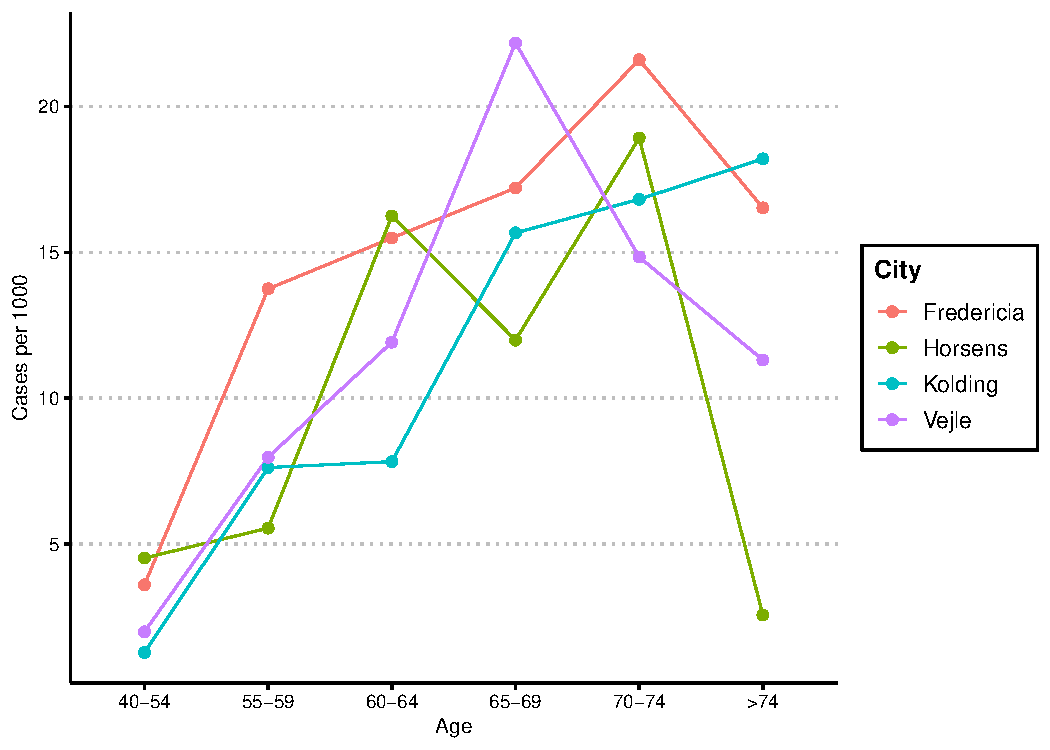
\includegraphics[width=0.9\textwidth]{plot_01.pdf}
    \end{center}
    \caption{
        Number of cases of lung cancer per 1000 people by age group and city.
    }
    \label{fig:danishlc}
    \end{figure}


    \section{Generalized linear models, Poisson family}

    The Poisson distribution is relevant here, for modelling the number of such rare
    events occurring in a given time period. Thus, we use the generalized linear
    model \[
        \log(\mu_i) = \bm{x}_i\bm{\beta} + \log(T_i).
    \] where $\mu_i$ is the corresponding expected number of cases in the age group
    $i$ and $T_i$ is the corresponding population. We also denote $y_i$ to be the
    actual number of cases in group $i$. Therefore, we model the expected case rate
    $\mu_i / T_i$ using a logarithmic link function, and appropriately chosen
    explanatory variables $\bm{x}_i$. The values $\log(T_i)$ act as \emph{offsets}.

    The null deviance of such a model, i.e.\ the deviance where only an intercept
    term is fitted, is $129.91$, with $23$ degrees of freedom.


    \subsection{Age group $*$ City}

    Here, the age group and city are treated as categorical explanatory variables,
    \emph{along with all interaction terms}. In the syntax of R, the model looks like
    \[
        \log(y_i) \;\sim\; \text{Age group } * \text{ City}
        + \text{offset}(\log(T_i)). \tag{i}
    \] Since there are essentially as many parameters as there are data points, this
    model has zero degrees of freedom, hence exhibits a residual deviance of zero.
    The fitted response is precisely the same as the supplied data points. Since this
    model is of little interest, we do not list the (23) model parameters here, nor
    do we show the predicted response graph (which coincides with
    Figure~\ref{fig:danishlc}).


    \subsection{Age group}

    Here, the age group is treated as a categorical explanatory variable, giving the
    model \[
        \log(y_i) \;\sim\; \text{Age group}  + \text{offset}(\log(T_i)). \tag{ii}
    \] This model yields a residual deviance of $28.31$, with 18 degrees of freedom.

    \begin{verbatim}
                            Estimate Std. Error z value Pr(>|z|)    
                (Intercept) -4.45397    0.17961 -24.799  < 2e-16 ***
                Age40-54    -1.40828    0.25012  -5.630  1.8e-08 ***
                Age55-59    -0.32594    0.25201  -1.293   0.1959    
                Age60-64     0.09339    0.23561   0.396   0.6918    
                Age65-69     0.34201    0.23341   1.465   0.1429    
                Age70-74     0.43894    0.23929   1.834   0.0666 .  
    \end{verbatim}


    \subsection{Age (numeric)}

    Here, the lower bound of an age group is treated as a numeric explanatory
    variable, giving the model \[
        \log(y_i) \;\sim\; \text{Age} + \text{offset}(\log(T_i)). \tag{iii}
    \] This model yields a residual deviance of $65.32$, with 22 degrees of freedom.

    \begin{verbatim}
                            Estimate Std. Error z value Pr(>|z|)    
                (Intercept) -5.63185    0.14058 -40.062  < 2e-16 ***
                AgeLower     0.28459    0.03498   8.135 4.11e-16 ***
    \end{verbatim}


    \subsection{Age (numeric, quadratic)}

    Here, the lower bound of an age group is treated as a numeric explanatory
    variable and used to fit a quadratic polynomial, giving the model \[
        \log(y_i) \;\sim\; \text{Age} + \text{Age}^2 + \text{offset}(\log(T_i)).
        \tag{iv}
    \] This model yields a residual deviance of $29.373$, with 21 degrees of freedom.

    \begin{verbatim}
                               Estimate Std. Error z value Pr(>|z|)    
            (Intercept)        -4.60357    0.06733 -68.369  < 2e-16 ***
            poly(AgeLower, 2)1  2.30787    0.34658   6.659 2.76e-11 ***
            poly(AgeLower, 2)2 -1.90891    0.32672  -5.843 5.14e-09 ***
    \end{verbatim}


    \begin{figure}[H]
    \begin{center}
        \vspace{1em}
        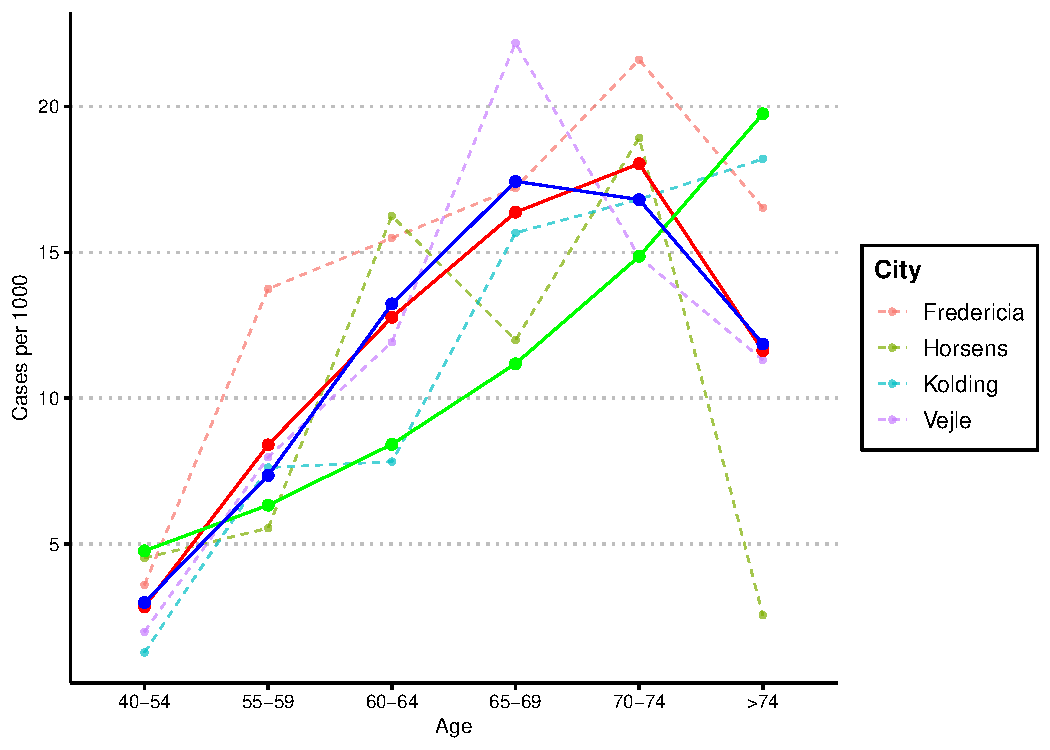
\includegraphics[width=0.9\textwidth]{plot_06.pdf}
    \end{center}
    \caption{
        Predicted number of cases of lung cancer per 1000 people according to models
        (ii) in \textcolor{red}{red}, (iii) in \textcolor{green}{green}, and (iv) in
        \textcolor{blue}{blue}. The actual data is shown with dashed lines. Note that
        the predictions are independent of the city (by design).
    }
    \label{fig:danishlc_glm}
    \end{figure}


    \section{Model selection}

    We may immediately discard model (i), as it overfits the available data, leaving
    no real way of judging its predictive power. Furthermore, we may discard model
    (iii) as the predicted trend in Figure~\ref{fig:danishlc_glm} is visibly not
    reflected in the data.

    Models (ii) and (iv) offer very similar predictions, hence very similar residual
    deviances. On the other hand, model (ii) requires the estimation of 6 parameters,
    while model (iv) requires only 3. Moreover, only 2 of the 6 parameters in model
    (ii) are non-zero with a satisfactory level of significance ($p < 0.05$).

    Thus, we are lead to choose model (iv), which is the simplest model that manages
    to capture the overall trend in the data.


    \section{Discussion}

    Both the data (Figure~\ref{fig:danishlc_box}) and our model suggest that there is
    a steady increase in the rate of occurrence of lung cancer from the ages of 40 to
    around 65 years, after which it decreases! It must be noted that these age groups
    reflect the time of \emph{diagnosis} of lung cancer, which can remain undetected
    for years. This introduces a certain bias in our data; people in the age groups
    of 65-75 years are perhaps more likely to present symptoms, or undergo more
    regular screenings. This may also help explain the dip in lung cancer incidence
    in the 75+ age group. Another possibility is that lung cancer may be one of
    several maladies affecting this age group, which consequently remains unnoticed
    altogether.


    \begin{figure}[H]
    \begin{center}
        \vspace{1em}
        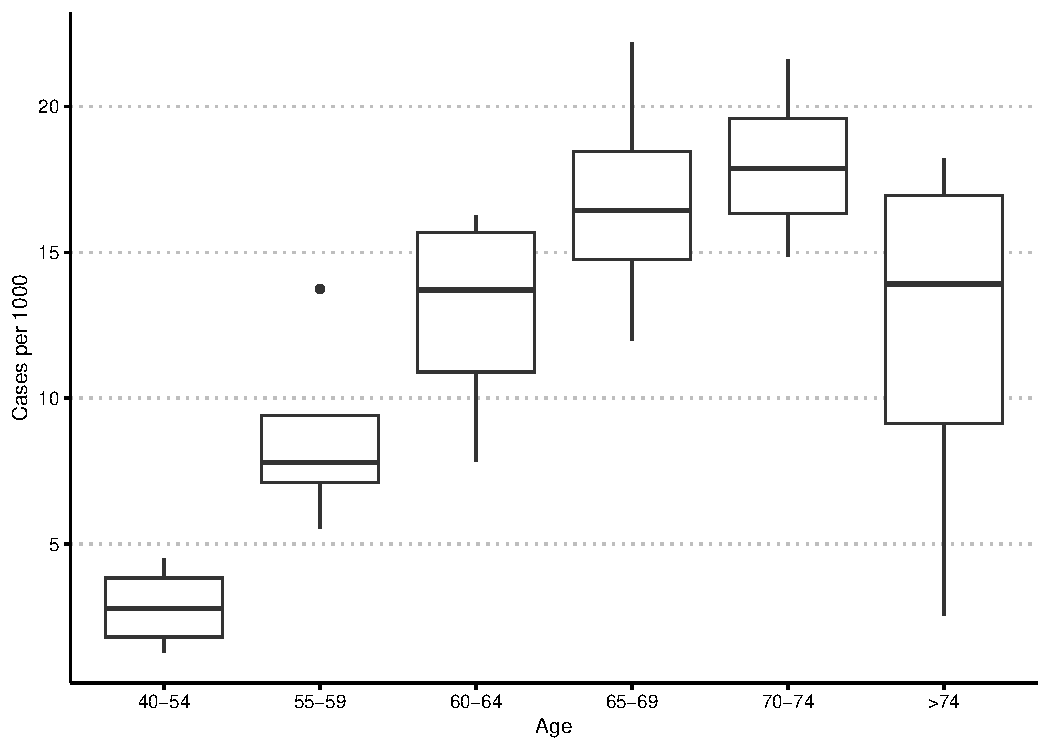
\includegraphics[width=0.9\textwidth]{plot_07.pdf}
    \end{center}
    \caption{
        Number of cases of lung cancer per 1000 people by age group.
    }
    \label{fig:danishlc_box}
    \end{figure}

    Here, we have not invoked the deviance measure \[
        D_{\text{null}} - D_{\text{residual}} \;\sim\; \chi_{n - m}^2,
    \] where the null model has $p$ degrees of freedom and the proposed model has $n$
    degrees of freedom, to distinguish between our models and the \emph{saturated}
    model since the corresponding $p$-values are essentially zero in all four cases.

    If we had to compare models (iii) and (iv), say to determine the significance of
    the quadratic term, we may have examined the difference in residual deviances and
    tested it against a $\chi_1^2$ distribution. However, the corresponding $p$-value
    is practically zero since this deviance measure exceeds 30.


\end{document}
